%% Los cap'itulos inician con \chapter{T'itulo}, estos aparecen numerados y
%% se incluyen en el 'indice general.
%%
%% Recuerda que aqu'i ya puedes escribir acentos como: 'a, 'e, 'i, etc.
%% La letra n con tilde es: 'n.

\chapter{Marco Te\'orico}
\section{Rob\'otica}
\subsection{Breve recorrido por la historia de la Rob\'otica}
La Rob\'otica fu\'e un t\'ermino acu\~nado por Isaac Asimov, el cual fue un escritor en su tiempo de ciencia ficci\'on, realidad en nuestra era. La rob\'otica tuvo sus inicios en la cultura griega, los cuales llamaban \emph{automatos} que era la palabra que ten\'ian para denominar a sus m\'aquinas, de esta palabra deriva \emph{automata}.\\
Los \'arabes (siglo VII a XV) utilizaron los conocimientos griegos para realizar m\'aquinas que ya no solo las usaban para su diversi\'on sino que comenzaron a darle aplicaciones pr\'acticas un ejemplo de ello eran los dispensadores de agua autom\'aticos. \\
Durante los siglos XVII y XVIII  se crearon algunas m\'aquinas con forma similar a los humanos y algunos animales, estos dispositivos creados en la mayor\'ia por el gremio de relojeros se utilizaban para la diversion y entretenimiento. \\
A finales del siglo VIII y principios del XIX se crearon algunas invenciones mec\'anicas como la hiladora giratoria de Hargreaves(1770), el telar mec\'anico de Cartwright (1785) y el telar de Jacquard (1801).\\
En 1948 R.C. Goertz del \emph{Argonne National Laboratory} desarrollo, el primer telemanipulador con el objetivo de manipular los elementos reactivos sin riesgo a los operadores humanos, este es el antecedente m\'as cercano a los robots, desp\'ues estos telemanipuladores evolucionaron y luego ya se hablaba de robots, cuyas primeras configuraciones eran como de esferas y antropom\'orficas. En 1982 El profesor Makino de la Universidad Yamanashi de Japon desarrolla el robot SCARA (\emph{Selective Compliance Assembly Robot Arm}) cuyo principal objetivo era el de ensabamblado de piezas en cadenas de produccion industriales. \cite{lib_rob1}.\\
En la Tabla a continuaci\'on podemos ver una breve linea del tiempo de los sistemas llamados Automatas durante el tiempo, anteriormente citados.\\\\


\begin{tabular}{|c|l|l|}
\hline 
\textbf{A\~no} & \textbf{Auto}r & \textbf{Aut\'omata} \\ 
\hline 
1352 & Desconocido & Gallo de la catedral de Estrasburgo \\ 
\hline 
1499 & L.Da Vinci & Le\'on Mec\'anico \\ 
\hline 
1525 & J. Turriano & Hombre de Palo \\ 
\hline 
1738 & J de Vaucanson & Flautista, tamborillero, pato \\ 
\hline 
1769 & W. Von Kempelen & Jugador de Ajedrez \\ 
\hline 
1770 & Familia Droz & Escriba, organista, dibujante \\ 
\hline 
1805 & H.Maillardet & Mu\~neca mecanica dibujante \\ 
\hline 
\end{tabular}
\subsection{Definicion de Rob\'otica y Sistema Rob\'otico}
La definicion de rob\'otica es la ciencia de estudio de la conexi\'on inteligente entre la percepcion y accion. Com\'unmente un sistema rob\'otico es un sistema complejo compuesto por m\'ultiples subsistemas (Fig 3.1). \\
La capacidad de un robot para poder ejecutar una accion viene dada por el \textit{Sistema de Actuadores} el cual anima los componentes mec\'anicos del robot. La capacidad de percibir el mundo exterior esta dado por el \textit{Sistema de Sensores} el cual modifica el estado interior del sistema mecanico tomando datos del mundo exterior. La capacidad de conectar la accion con la percepci\'on viene dada por el \textit{Sistema de Control} el cual ejecuta comandos siguiendo las reglas de la tecnica de planificaci\'on del robot.\cite{lib_rob2}
\begin{figure}
\centering
\includegraphics[width=3.0in]{imagen3.pdf}
\caption{Subsistemas dentro de un robot (Fuente: Elaboraci\'on Propia)}
\label{fig_mar}
\end{figure}

%%%%%%%%%%%%%%% ACA PUEDE IR ESA TABLA DEL LIBRO
 \section{Redes Neuronales}
 Las redes neuronales artificiales son estructuras paralelas las cuales se acercan al comportamiento de las redes neuronales humanas. Estan compuestas por neuronas  interconectadas mediantes axones donde varias neuronas pueden formar una capa (si se tratara de una red neuronal multicapa), y varias capas formar una neurona.\\
 Podemos explicar una red neuronal con salida binaria en la figura 3.2:\\
 
 \begin{figure}
\centering
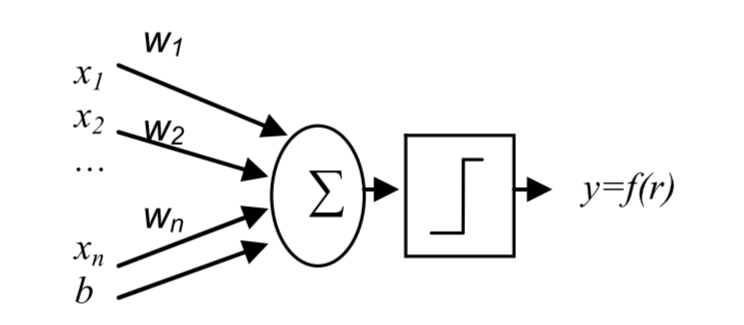
\includegraphics[width=3.0in]{imagen4.pdf}

\caption{Red Neuronal de Salida Binaria}
\label{fig_mar}
\end{figure}
Donde $x_1,x_2,x_3,...,x_n$ son las entradas para la red neuronal,$w_1,w_2,w_3,...,w_n$  son los pesos sinapticos, y $b$ es un factor de polarizaci\'on. El resultado final de la funci\'on se calcular asi: 
\begin{equation}
r= \sum_{i=1}^{n}x_iw_i+b
\end{equation}
El resultado de esta ecuaci\'on  nos dar\'a 1 o 0 y si se tratara de una red multicapa este seria la entrada para otra red neuronal.\cite{art_red1}

 \section{Procesamiento de Im\'agenes}
El procesamiento de im\'agenes es utilizado para mejorar las imagenes,prepararlas correctamente para un an\'alisis por parte de m\'aquinas. Consta de 4 procesos basicamente.\cite{art_red1}
\begin{enumerate}
\item Preprocesamiento: Son operaciones para adaptar la informaci\'on de una imagen y tenerla lista para el siguiente paso. Por ejemplo cambiar el brillo, reducir ruido.
\item Segmentacion: Separar la imagen en partes de las cuales se pueda hacer un analisis independiente.
\item Deteccion de objetos y clasificacion: Determinar cual objetos es cual.
\item Analisis de Imagen Obtener Informacion de alto nivel acerca de la imagen.
\end{enumerate}
 \begin{figure}
	\centering
	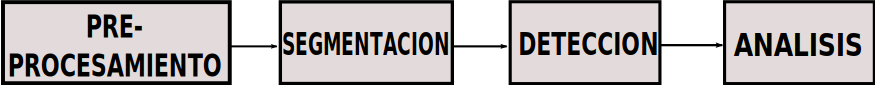
\includegraphics[width=3.0in]{imagen5.pdf}
	\caption{Pasos del Procesamiento de Im\'agenes(Fuente: elaboraci\'on propia)}
	
	%%\label{fig_mar}
\end{figure}
% \subsection{Vision Artificial}
 %\subsection{Seguimiento de Objetos}